
\documentclass{article}
\title{Reading Notes for ch8 Graphical Models}
\author{Xiang Pan}

\usepackage{url}
\usepackage{titling}
\usepackage{geometry}

\geometry{a4paper,scale=0.8}
\usepackage{amsmath}
\usepackage{hyperref}
\usepackage{amsfonts}
\usepackage{tikz}
% \usepackage{unicode-math}
\def\ci{\perp\!\!\!\perp}
\usetikzlibrary{fit,positioning}
\usepackage{multicol} % for multi column 

\hypersetup{
    colorlinks=true,
    linkcolor=blue,
    filecolor=blue,      
    urlcolor=blue,
    citecolor=cyan,
}


\begin{document}
\maketitle
\section{Graphical Models}
We can trun the probability dependency of a random variable to a graphical model.

Note: We use the notations from the bishop book.
\begin{align}
p(\mathbf{w} \mid \mathbf{T}) \propto p(\mathbf{w}) \prod_{n=1}^{N} p\left(t_{n} \mid \mathbf{w}\right)
\end{align}


% \begin{figure}
%     \centering
%     \begin{tikzpicture}
        
%     \tikzstyle{main}=[circle, minimum size = 10mm, thick, draw =black!80, node distance = 16mm]
%     \tikzstyle{connect}=[-latex, thick]
%     \tikzstyle{dot}=[-latex, dotted]
%     % \tikzstyle{box}=[rectangle, draw=black!100]
%       \node[main] (w) [label=below:$w$] { };
%       \node[main] (t1) [below=of w, label=below:$t1$] { };
%       \node[main] (tn) [right=of t1, label=below:$tn$] { };
%     %   \node[main] (theta) [right=of alpha,label=below:$\theta$] { };
%     %   \node[main] (z) [right=of theta,label=below:z] {};
%     %   \node[main] (beta) [above=of z,label=below:$\beta$] { };
%     %   \node[main, fill = black!10] (w) [right=of z,label=below:w] { };
%       \path (w) edge [connect] (t1);
%       \path (w) edge [connect] (tn);
%       \path (t1) edge [dotted] (tn);
%     %         (theta) edge [connect] (z)
%     %         (z) edge [connect] (w)
%     %         (beta) edge [connect] (w);
%     %   \node[rectangle, inner sep=0mm, fit= (z) (w),label=below right:N, xshift=13mm] {};
%     %   \node[rectangle, inner sep=4.4mm,draw=black!100, fit= (z) (w)] {};
%     %   \node[rectangle, inner sep=4.6mm, fit= (z) (w),label=below right:M, xshift=12.5mm] {};
%     %   \node[rectangle, inner sep=9mm, draw=black!100, fit = (theta) (z) (w)] {};
%     \end{tikzpicture}
% \end{figure}


\begin{figure}[htbp]
    \centering
    \begin{minipage}[t]{0.48\textwidth}
    \centering
    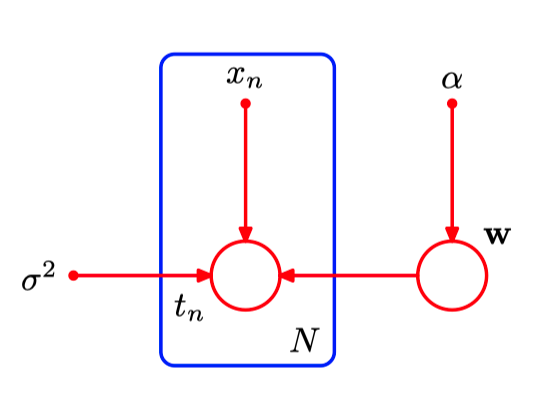
\includegraphics[width=4cm]{./images/2021-09-15-17-09-32.png}
    \caption{Graphical Model of observation} 
    \end{minipage}
    \begin{minipage}[t]{0.48\textwidth}
    \centering
    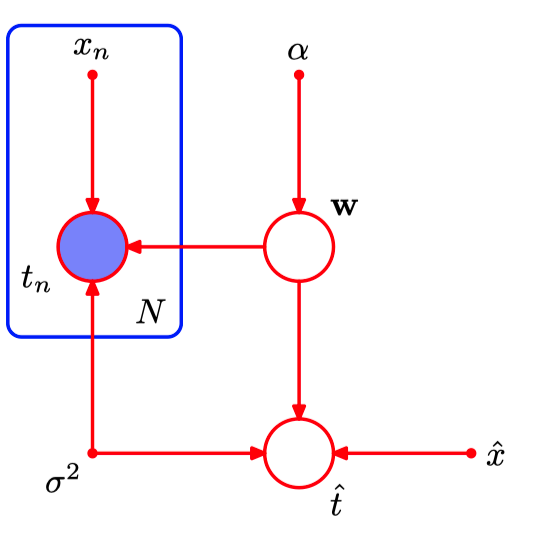
\includegraphics[width=3cm]{./images/2021-09-15-17-15-12.png}
    \caption{Prediction}
    \end{minipage}
\end{figure}
  

% \begin{figure}[!htb] 
% \centering 
% \includegraphics[width=0.2\textwidth]{} 
% \caption{The graphic model of regression}
% \label{Fig.main2} 
% \end{figure}



\begin{align}
    p\left(\widehat{t}, \mathbf{t}, \mathbf{w} \mid \widehat{x}, \mathbf{x}, \alpha, \sigma^{2}\right)=\left[\prod_{n=1}^{N} p\left(t_{n} \mid x_{n}, \mathbf{w}, \sigma^{2}\right)\right] p(\mathbf{w} \mid \alpha) p\left(t \mid \widehat{x}, \mathbf{w}, \sigma^{2}\right)
\end{align}

\begin{equation}
    p\left(t \mid \widehat{x}, \mathbf{x}, \mathbf{t}, \alpha, \sigma^{2}\right) \propto \int p\left(\widehat{t}, \mathbf{t}, \mathbf{w} \mid \widehat{x}, \mathbf{x}, \alpha, \sigma^{2}\right) \mathrm{d} \mathbf{w}
\end{equation}

% \begin{figure}[!htb] 
%     \centering 
%     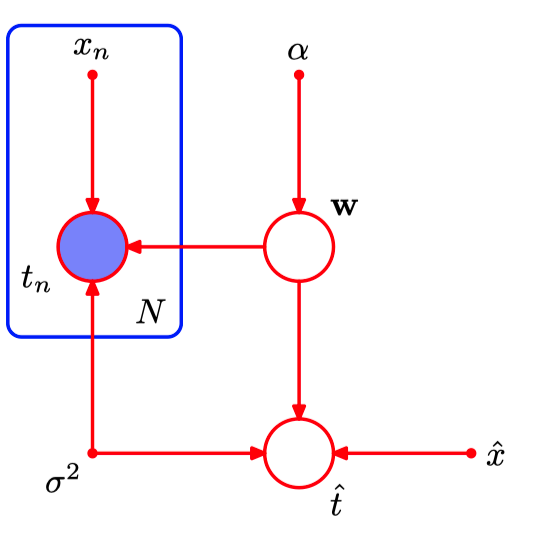
\includegraphics[width=0.2\textwidth]{./images/2021-09-15-17-15-12.png} 
%     \caption{The graphic model of regression for prediction}
%     \label{Fig.main2} 
% \end{figure}

An alternative way to reduce the number of independent parameters in a model is by sharing parameters (also known as tying of parameters).
\section{Conditional Independence}
\footnote{You can get the full version note at \\\url{https://github.com/Xiang-Pan/NYU_Bayesian_Machine_Learning/blob/master/reading_notes/ch8/build/note4.pdf}}
Conditional Independence is widely used in causal learning \cite{pearl2016causal}. We use the name of three types of conditional independence in causal learning.
\begin{figure}[!htb]
    \centering
    \begin{minipage}[t]{0.32\textwidth}
        \centering
        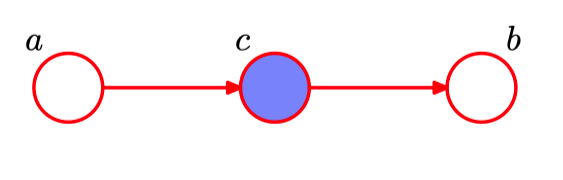
\includegraphics[width=2cm]{./images/2021-09-15-17-49-28.png}
        \caption{V-Structure \\ (Chain Structure)}
    \end{minipage}
    \begin{minipage}[t]{0.32\textwidth}
        \centering
        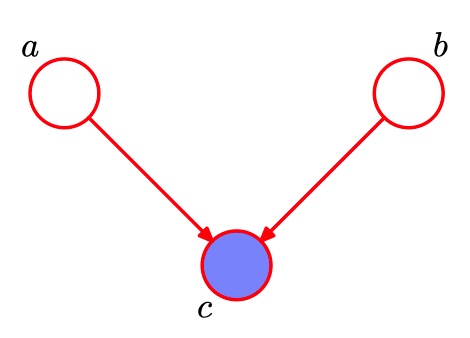
\includegraphics[width=2cm]{./images/2021-09-15-17-43-00.png}
        \caption{Collider Structure} 
    \end{minipage}
    \begin{minipage}[t]{0.32\textwidth}
        \centering
        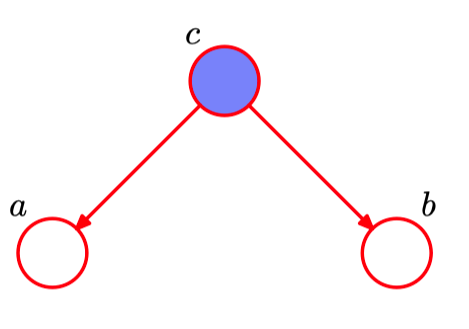
\includegraphics[width=2cm]{./images/2021-09-15-17-43-54.png}
        \caption{Fork Structure}
    \end{minipage}
\end{figure}

\newpage
\begin{multicols}{3}       % 分两栏 若花括号中为3则是分三列
    \textbf{V-Structure}
    \begin{equation}
        p(a, b, c)=p(a) p(c \mid a) p(b \mid c)
    \end{equation}
    
    \begin{equation}
        a \not \ci b \mid \emptyset
    \end{equation}
    
    \begin{equation}
        \begin{aligned}
        p(a, b \mid c) &=\frac{p(a, b, c)}{p(c)} \\
        &=p(a \mid c) p(b \mid c)
        \end{aligned}
    \end{equation}
    
    \begin{equation}
        a  \ci b \mid c
    \end{equation}
    
    \textbf{Collider Structure}
    \begin{equation}
        p(a, b)=p(a) p(b)
    \end{equation}
    
    \begin{equation}
        a \ci b \mid \emptyset
    \end{equation}
    
    \begin{equation}
        \begin{aligned}
        p(a, b \mid c) &=\frac{p(a, b, c)}{p(c)} \\
        &=\frac{p(a) p(b) p(c \mid a, b)}{p(c)}
        \end{aligned}
    \end{equation}
    
    \begin{equation}
        a \not \ci b \mid c
    \end{equation}
    
    \textbf{Fork Structure}
    \begin{equation}
        p(a, b)=\sum_{c} p(a \mid c) p(b \mid c) p(c)
    \end{equation}
    
    \begin{equation}
        a \not \ci b \mid c
    \end{equation}
    
    
    \begin{equation}
        \begin{aligned}
        p(a, b \mid c) &=\frac{p(a, b, c)}{p(c)} \\
        &=p(a \mid c) p(b \mid c)
        \end{aligned}
    \end{equation}
    \begin{equation}
        a \ci b \mid c
    \end{equation}
\end{multicols}


\section{D-Separation}
Consider a general directed graph in which A, B, and C are arbitrary nonintersecting sets of nodes. To evaluate whether $A \ci B | C$, we consider all possible paths from any node in A to any node in B:
blocked paths:
\begin{itemize}
    \item[(a.)] the arrows on the path meet either head-to-tail or tail-to-tail at the node, and the node is in the set C, or
    \item[(b.)]the arrows meet head-to-head at the node, and neither the node, nor any of its descendants, is in the set C.
\end{itemize}
If all paths are blocked, then A is said to be d-separated from B by C, and the joint distribution over all of the variables in the graph will satisfy $A \ci B | C$.
In summary, observation (given exact value) will block the path.

% \section{Markov Random Fields}
% We can easily factorize directed graphs,
% \begin{equation}
%     p(x)=\prod_{i=1}^{p} p\left(x_{i} \mid x_{prior^{(i)}}\right)
% \end{equation}
% \subsection{Conditional Independence}
% \textbf{Global Markov}
% \textbf{Local Markov}
% \textbf{Local Markov}
% Markov Random Fields (MRF) 


% \section{Inference in Graphical Models}


\bibliographystyle{plain}
\bibliography{note4}
\appendix
\end{document}